%%
% The BIThesis Template for Bachelor Graduation Thesis
%
% 北京理工大学毕业设计(论文) —— 使用 XeLaTeX 编译
%
% Copyright 2021-2023 BITNP
%
% This work may be distributed and/or modified under the
% conditions of the LaTeX Project Public License, either version 1.3
% of this license or (at your option) any later version.
% The latest version of this license is in
%   http://www.latex-project.org/lppl.txt
% and version 1.3 or later is part of all distributions of LaTeX
% version 2005/12/01 or later.
%
% This work has the LPPL maintenance status `maintained'.
%
% The Current Maintainer of this work is Feng Kaiyu.
%
% Compile with: xelatex -> biber -> xelatex -> xelatex

% 开启盲审格式 blindPeerReview=true (如:[type=bachelor,blindPeerReview=true])

\documentclass[type=bachelor]{bithesis}

\BITSetup{
  cover = {
    % 在封面中载入有「北京理工大学」字样的图片,如无必要请勿改动。
    headerImage = images/header.png,
    % 在封面标题中使用思源黑体,使用此选项可以保证与 Word 封面标题的字体一致。
    xiheiFont = STXIHEI.TTF,
    %% 使用以下参数来自定义封面日期
    % date = 2022年6月,
  },
  info = {
    % 想要删除某项封面信息,直接删除该项即可。
    % 想要让某项封面信息留空(但是保留下划线),请设置为空字符串。
    % 如需要换行,则用 “\\” 符号分割。
    title = 基于深度学习的端到端多实例点云配准,
    titleEn = {Deep Learning Based End-To-End Multi-instance  Point Cloud Registration},
    school = \quad 自动化学院 \quad,
    major = 自动化,
    author = 杨润一,
    class = 06111902,
    studentId = 1120191211,
    supervisor = 由育阳,
    keywords = {点云配准; 多实例; 聚类; 对应聚类; 深度学习},
    keywordsEn = {Point Cloud Registration; Multi-instance; Clustering; Correspondence Clustering; Deep Learning},
    % 如果你的毕设为校外毕设,请将下面这一行语句解除注释(删除第一个百分号字符)并填写你的校外毕设导师名字
    % externalSupervisor = 左偏树,
  },
  style = {
    % 保持参考文献的缩进样式与 Word 模板一致。
    % 如果你不需要此样式,请将此行注释掉。
    bibliographyIndent = false,
  }
}

% 使用 listings 宏包进行代码块使用,并使用了预定义的样式,
% 你也可以选用自己的喜欢的其他宏包,如 minted;
% 然而由于 minted 依赖 Python 的 Pygments 库作为外部依赖,因此出于模板的简洁程度考虑,我们没有提供 minted 进行代码块书写的示例。
\usepackage{listings}

\usepackage[
  backend=biber,
  style=gb7714-2015,
  gbalign=gb7714-2015,
  gbnamefmt=lowercase,
  gbpub=false,
  doi=false,
  url=false,
  eprint=false,
  isbn=false,
]{biblatex}

% 参考文献引用文件位于 misc/ref.bib
\addbibresource{misc/ref.bib}


% 文档开始
\begin{document}

% 标题页面:如无特殊需要,本部分无需改动
\MakeCover

% 原创性声明:如无特殊需要,本部分无需改动
% 更改为 PDF 页面插入,如需要添加内容,可考虑先用 Word 制作再覆盖 misc/1_originality.pdf
% ====== 原创性声明(PDF 格式)======
\begin{blindPeerReview}
  
\includepdf{misc/1_originality.pdf}\newpage
\end{blindPeerReview}
% ====== 原创性声明(PDF 格式)======
% ====== 原创性声明(LaTeX 格式)======
% %%
% The BIThesis Template for Bachelor Graduation Thesis
%
% 北京理工大学毕业设计(论文)原创性声明模板 —— 使用 XeLaTeX 编译
%
% Copyright 2020-2023 BITNP
%
% This work may be distributed and/or modified under the
% conditions of the LaTeX Project Public License, either version 1.3
% of this license or (at your option) any later version.
% The latest version of this license is in
%   http://www.latex-project.org/lppl.txt
% and version 1.3 or later is part of all distributions of LaTeX
% version 2005/12/01 or later.
%
% This work has the LPPL maintenance status `maintained'.
%
% The Current Maintainer of this work is Feng Kaiyu.
%
% Compile with: xelatex -> biber -> xelatex -> xelatex
%
% 如无特殊需要,本页面无需更改

\MakeOriginality

% ====== 原创性声明(LaTeX 格式)======

% 前置页面定义
\frontmatter
% 摘要:在摘要相应的 TeX 文件处进行摘要部分的撰写
%%
% The BIThesis Template for Bachelor Graduation Thesis
%
% 北京理工大学毕业设计(论文)中英文摘要 —— 使用 XeLaTeX 编译
%
% Copyright 2020-2023 BITNP
%
% This work may be distributed and/or modified under the
% conditions of the LaTeX Project Public License, either version 1.3
% of this license or (at your option) any later version.
% The latest version of this license is in
%   http://www.latex-project.org/lppl.txt
% and version 1.3 or later is part of all distributions of LaTeX
% version 2005/12/01 or later.
%
% This work has the LPPL maintenance status `maintained'.
%  
% The Current Maintainer of this work is Feng Kaiyu.

% 中英文摘要章节
\begin{abstract}
    三维点云配准是点云处理中的一项基本任务,其在机械臂、自动驾驶、自主运动机器人、即时定位与地图构建(Simultaneous Localization and Mapping,SLAM)等众多基于视觉方法的应用中起着关键的作用。随着人工智能、元宇宙、自动驾驶等技术的兴起,将深度学习应用于点云配准的工作已经日趋成熟。目前大多数点云配准任务研究主要集中在成对配准上。然而,在实际应用中,目标场景可能包含多个重复实例,我们需要估计模板点云与目标点云中这些重复实例之间的多个刚性变换,也就是多实例点云配准。

    本文针对三维点云配准问题,特别是多实例点云配准,进行了深入研究。我们调研并整理了多实例点云配准的国内外研究现状,并总结了前人研究的优势和劣势。现有解决方案需要对大量假设进行采样以检测可能的实例并排除异常值,当实例和异常值的数量增加时,其鲁棒性和效率会显着降低。我们建议根据距离不变矩阵将噪声对应集直接分组到不同的簇中。通过聚类自动识别实例和异常值,达到稳健且快速表现。
    
    基于这一研究背景,我们提出了新的多实例点云配准架构,高效对应聚类的多实例点云配准 (ECC) 。分析聚类方法的点云配准,发现对于描述子的依赖性高,离群点比例高的时候效果会大大下降,所以我们提出了基于深度学习和聚类优化的多实例点云配准 (DMR),首先利用对比学习来学习输入推定对应关系的分布良好的深度表示。然后基于这些表示,我们提出了异常值修剪策略和聚类策略,以有效地删除异常值并将剩余的对应关系分配给正确的实例,达到了更好的效果。
    
    综上所述,我们的研究表明,基于深度学习的多实例点云配准方法在处理复杂的多实例点云配准问题上具有优秀的性能,提供了新的研究思路和方法。
    
\end{abstract}

% 英文摘要章节
\begin{abstractEn}
    Three-dimensional point cloud registration is a fundamental task in point cloud processing, which plays a crucial role in a wide range of vision-based applications such as robotic arms, autonomous driving, autonomous mobile robots, and Simultaneous Localization and Mapping (SLAM). With the rise of artificial intelligence, metaverse, autonomous driving, and other technologies, the application of deep learning to point cloud registration has become increasingly mature. Current research on point cloud registration mostly focuses on pairwise registration. However, in practical applications, the target scene may contain multiple repeated instances, and we need to estimate multiple rigid transformations between the template point cloud and these repeated instances in the target point cloud, that is, multi-instance point cloud registration.

    This paper conducts in-depth research on the problem of three-dimensional point cloud registration, especially multi-instance point cloud registration. We have surveyed and summarized the domestic and international research status of multi-instance point cloud registration and summarized the advantages and disadvantages of previous studies. Existing solutions require sampling a large number of hypotheses to detect possible instances and reject outliers, and their robustness and efficiency degrade significantly when the number of instances and outliers increases. We propose to directly group the noisy correspondence set into different clusters based on a distance invariance matrix. Through clustering, instances and outliers are automatically identified, achieving robust and fast performance.
    
    Based on this research background, we propose a new multi-instance point cloud registration framework, \textbf{E}fficient \textbf{C}orrespondence \textbf{C}lustering for Multi-instance Point Cloud Registration (\textbf{ECC}). After analyzing the point cloud registration of the clustering method, we find that the effect will drop significantly when it has high dependency on the descriptor and a high proportion of outliers. Therefore, we propose \textbf{D}eep Learning and Cluster Opimisation based \textbf{M}ulti-instance Point Cloud \textbf{R}egistration (\textbf{DMR}), which first uses contrastive learning to learn a good deep representation of the input estimation correspondence. Then, based on these representations, we propose an outlier pruning strategy and a clustering strategy to effectively remove outliers and allocate the remaining correspondences to the correct instances, achieving better results.
    
    In conclusion, our research shows that the deep learning-based multi-instance point cloud registration method has excellent performance in dealing with complex multi-instance point cloud registration problems and provides new research ideas and methods.
\end{abstractEn}


\MakeTOC

% 正文开始
\mainmatter

% 第一章
%%
% The BIThesis Template for Bachelor Graduation Thesis
%
% 北京理工大学毕业设计(论文)第一章节 —— 使用 XeLaTeX 编译
%
% Copyright 2020-2023 BITNP
%
% This work may be distributed and/or modified under the
% conditions of the LaTeX Project Public License, either version 1.3
% of this license or (at your option) any later version.
% The latest version of this license is in
%   http://www.latex-project.org/lppl.txt
% and version 1.3 or later is part of all distributions of LaTeX
% version 2005/12/01 or later.
%
% This work has the LPPL maintenance status `maintained'.
%
% The Current Maintainer of this work is Feng Kaiyu.
%
% 第一章节

\chapter{绪论}

\section{研究背景和意义}
% 这里插入一个参考文献,仅作参考

\subsection{三维点云配准}
21世纪以来,人工智能技术的发展对于社会有着重大的影响,智能化成为工程技术突破的内核。机器能够进行快速计算、存储和处理大量数据,并通过互联网将社会连为一体。现在由人工智能驱动的新一代机器,它们可以越来越自主地解决复杂的任务,其中以视觉为核心的机器技术快速发展,机械臂、自动驾驶、自主运动机器人等进入了人们的视野。随着2012年AlexNet\cite{krizhevsky2017imagenet} 问世以来,深度学习方法打开了计算机视觉的新大门。越来越多的深度学习方法比如VGG\cite{simonyan2014very} 、ResNet\cite{he2016deep} 、ViT\cite{dosovitskiy2020image} 被用在了图像分类、分割、场景理解等任务中。为了更好的理解真实世界,人们开始尝试将深度学习方法用于三维数据中,随着激光雷达和Kinect等高精度传感器的快速发展,点云已经成为表示三维世界的主要数据格式。2017年PointNet\cite{qi2017pointnet} 出现后,深度学习方法也同样被广泛应用在了点云处理中。

三维点云配准是点云处理中的一项基本任务\cite{qi2017pointnet,huang2021comprehensive,besl1992method} ,其在机械臂、自动驾驶、自主运动机器人等众多基于视觉方法的应用中起着关键的作用。首先是三维重建,生成完整的三维场景是各种计算机视觉应用的基础和重要技术,包括自动驾驶中的高精度三维地图重建、机器人技术中的三维环境重建等。例如,配准可以为机器人应用程序中的路线规划和决策构建三维环境。

其次,三维场景中的定位。三维场景中的定位和重定位对于机器人技术尤其重要。例如,无人驾驶汽车会估计其在地图上的位置及其与道路边界线的距离。点云配准可以将当前的实时三维视图与其所属的三维环境准确匹配,提供高精度定位服务。此应用表明,点云配准提供了机器和三维环境交互一种解决方案。

第三,位姿估计。将点云A与另一个点云B对齐可以生成与点云B相关的点云A的位姿信息。这个位姿信息可用于机器人决策。例如,点云配准可以获取环境中物体的位姿信息,以决定机械臂移动到哪里以准确抓取并移动物体。位姿估计为机器人三维环境理解提供了重要信息。

在国防安全、信息安全、环境安全等领域,无人机系统、自主导航、环境感知等技术应用愈发广泛。在这些应用中,点云配准也发挥着重要作用。例如,无人机系统需要对目标进行跟踪,而点云配准可以提供目标的位姿信息,来实现目标跟踪。点云配准可以用于环境感知,用于分割、检测、识别等任务,从而实现环境感知。在自动驾驶、机器人自主导航中,高精度的点云配准算法可以提供高精度的3D地图场景重建,为自主机器提供视觉定位、路径规划、障碍物检测等技术保障\cite{zidongjiashilujingguihua} 。


\subsection{多实例点云配准}
点云配准旨在通过对源点云和目标点云之间进行刚性变换,使得源点云和目标点云尽可能重合。点云配准的输入是两个点云,输出是一个刚性变换矩阵。点云配准的目标是找到一个刚性变换矩阵,使得源点云和目标点云之间的距离最小。传统方法中,一般流程为查找匹配点,通过SVD等方法求解出变换矩阵。随着机器学习和深度学习算法的广泛使用,基于深度学习方法和组合优化方法进一步提高了点云配准的准确率\cite{deng2018ppf,deng2018ppfnet,qin2022geometric} 。

\begin{figure*}[ht]
    \vspace{-4mm}
    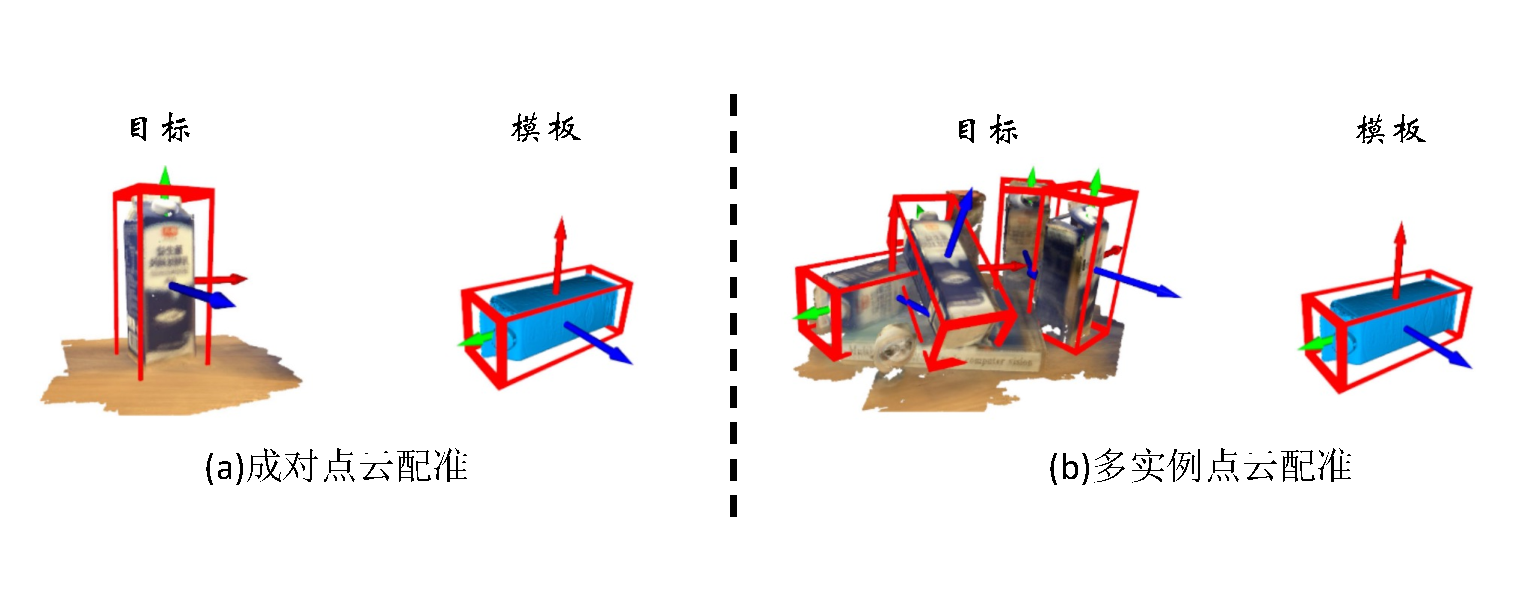
\includegraphics[width=\textwidth]{images/teaser.pdf}
    \caption{\textbf{多实例点云配准: } 给定目标的模板点云,成对点云配准(左)侧重于估计模板点云和目标点云之间的单个刚性变换,而多实例点云配准(右)旨在估计目标点云中相同物体的6D位姿。
    }
    \label{fig:teaser}
    \vspace{-10mm}
\end{figure*}

目前大多数点云配准任务研究主要集中在成对配准上。然而,在实际应用中,目标场景可能包含多个重复实例,我们需要估计模板点云与目标点云中这些重复实例之间的多个刚性变换。比如说在室内场景中,我们希望机器人能够将屋子中所有的椅子摆正,那么首先需要将多个椅子点云和模板椅子点云进行配准,求的目标椅子的位姿,通过机械运动来达到位姿改变的效果。图 \ref{fig:teaser} 展示了了一个示例。这个问题被命名为多实例点云配准,它比成对点云配准更具挑战性。针对该任务已有的现有文献研究较少,扩展现有的点云配准方法来解决这个问题并非易事。多实例点云配准不仅需要从嘈杂的对应中拒绝异常值,还需要识别单个实例的异常值集,这使得它比传统的配准问题更具挑战性。

与传统的两两配准方法相比,多实例点云配准需要解决更复杂的问题,同时也具有更广泛的应用价值。比如,在大规模场景重建任务中,通常需要处理成千上万个点云数据。单纯采用两两配准的方法可能导致累积误差,从而影响重建结果的精度。因此,研究多实例点云配准算法具有重要的实际意义。在机械臂抓取任务中,多实例点云配准算法可以在全局范围内考虑点云之间的约束关系,有助于消除局部误差和噪声的影响,从而提高配准结果的鲁棒性 \cite{stuckler2012robust} 。

尽管多实例点云配准技术在近年来取得了显著的进展,仍然存在许多亟待解决的问题。例如,现存的多实例点云配准一般采用多任务的方式,也就是先对点云分割或者三维目标检测,然后进行两两点云配准,这样的方式需要先训练点云分割或者目标检测网络,泛化性差。并且如果见到了不存在先验的点云,下游的配准任务仍然会失效。所以,本文我们会对多实例点云配准进行研究,通过点云直接进行多实例点云配准,不需要先进行点云分割或者目标检测,从而提高多实例点云配准的泛化性。


\section{国内外研究现状}

\subsection{点云配准}
点云配准长期以来一直是计算机视觉和机器人领域的一项基本任务,大致可分为直接方法 \cite{besl1992method, pomerleau2015review} 和基于特征的方法 \cite{qi2017pointnet,huang2021predator,bai2021pointdsc} 。近年来,由于深度学习的发展,许多基于特征的方法取得了最先进的性能。这些方法通常通过特征匹配产生对应关系,然后移除异常值以稳健地估计转换。尽管深度特征 \cite{qi2017pointnet,huang2021predator,bai2021pointdsc, wang2022you} 发展迅速,但特征匹配生成的对应关系仍然包含异常值。因此,去除异常点在点云配准中具有重要意义。过去,已经提出了许多传统方法来去除异常值,包括基于RANSAC的方法 \cite{barath2021progressive,zhao2021progressive,barath2018graph} 、基于分支和边界的方法 \cite{kluger2020consac} 以及许多其他方法 \cite{huang2021predator,yang2020teaser} 。最近,一系列基于学习的方法 \cite{bai2020d3feat,yi2018learning} 被提出,并在异常值去除方面取得了显着的效果。
以上的方法都是基于成对点云配准来完成的。然而,与成对配准不同,一个实例的内点构成多实例点云配准中所有其他实例的异常值。这种伪异常值使得很难将上述二元分类模型直接推广到多实例点云配准的情况。
现有该问题解决方案包括采用目标检测方法或对目标点云应用实例分割,将多实例点云配准问题转化为多个成对点云配准问题,但是这种方法需要预先训练一个目标检测或者点云分割网络,这样的方法对于已有点云类别是有效的,但是对于未知的类别是不适用的。另一种解决方案是通过多模型拟合,但是现有的多模型拟合方法依赖于抽样有效假设,当模型数量或离群率变高时,会涉及大量的抽样步骤,使得这些算法的效率和鲁棒性急剧下降。

\subsection{三维目标检测和实例分割}
三维物体的目标检测和实例分割与多实例点云配准有着密切的关系。输入一帧点云,目标检测模型 \cite{qi2019deep} 可以用来对获取每个目标对象的边界框,三维实例分割 \cite{wang2018sgpn,han2020occuseg} 为每个点生成实例标签。

这样的方法产生的结果类似于多实例点云配准的结果,但是它们需要将特定对象或类别的先验训练到网络中。基于点云匹配的筛选和聚类方法来进行多实例点云配准通过直接将模板点云和目标点云中的多个实例对齐来处理两组点云,而不使用任何关于输入的点云的先验信息。

\subsection{多模型拟合}
多实例配准也可以通过多模型拟合来实现,其目的是根据多个模型生成的数据点来进行建模。例如在点云中拟合多个平面 \cite{barath2018multi} ,在运动分割中估计基本矩阵 \cite{hartley1997defense} ,在多实例点云配准中计算刚性变换 \cite{tang2022multi} 等。但是由于一个实例的正常值构成所有其他实例的离群值,所以多模型拟合比单模型拟合更具挑战性。

现有的多模型拟合方法大致可以分为两类。第一类按顺序拟合模型 \cite{barath2019progressive,barath2021progressive,kanazawa2004detection,kluger2020consac} ,通过重复采样和筛选模型来进行建模。比如,Progressive-X \cite{barath2019progressive} 和Progressive-X+ \cite{barath2021progressive} 使用了表现更好的Graph-cut RANSAC \cite{barath2018graph} 作为采样方法来生成假设。CONSAC \cite{kluger2020consac} 首次将深度模型引入多模型拟合中,使用类似PointNet \cite{qi2017pointnet} 的网络来引导采样。通过重复采样来恢复单个实例,从输入中删除正常值和,以顺序的方式来检测实例。

第二类模型同时拟合多个模型 \cite{tang2022multi,toldo2008robust,magri2016multiple,magri2014t,magri2015robust} 。许多基于偏好分析的方法 \cite{toldo2008robust,magri2015robust} 最初对一系列假设进行采样,然后根据假设的残差对输入点进行聚类。ECC \cite{tang2022multi} 利用点云刚性变换空间一致性 \cite{leordeanu2005spectral} 和以自下而上的方式基于距离不变矩阵对对应关系进行聚类。PointCLM \cite{yuan2022pointclm} 使用了一种新的深层表示方法来与空间一致性相结合,得到了更好的结果。

% 本项目希望基于旋转等变的描述子来实现性能的初步提升,希望在模型中加入更多的内在形状和几何信息。通过端到端的方法优化整个方法系统,实现更高的准确性和鲁棒性。
\section{论文结构安排}
本论文共分为6章。

第一章为绪论,本章主要阐述了三维点云配准研究的重要性、背景以及现有的研究进展。通过对国内外三维点云配准研究文献的梳理和调查,我们对该领域的发展轨迹和现状进行了总结,并分析了先前研究所展现出的优点与缺点。同时,我们也详细介绍了本研究所完成的主要任务和做出的关键贡献。考虑到过去的研究中仍存在未完全解决的问题和挑战,我们特别指出了本研究所应用的策略和解决方案。最后,我们规划了清晰的文章结构,以引导读者理解本研究的整体框架。

在第二章,我们主要阐述了三维点云的基本数据格式和在本研究中所涉及的基础数学知识。同时,我们对在本研究中所用到的关于三维刚体变换的基础知识进行了详尽的总结和描述。

第三章在介绍了主要的数据集和评价指标后,引出深度学习方法在三维点云配准领域的研究与应用,并结合深度学习在三维点云配准领域做出的代表性工作 PointNet \cite{qi2017pointnet} 和 PointNet++ \cite{qi2017pointnet++} 进行介绍,并介绍和使用 PREDATOR \cite{huang2021predator} 作为骨干网络提取点云的点对特征供后续使用。

第四章主要介绍了本文提出的多实例点云配准,首先我们根据点云的特征进行聚类,然后对每个聚类进行对应聚类,最后进行刚性变换估计;其次,我们引入深度学习的方法,学习鲁棒的点对特征,进行谱聚类,得到了点云配准更好的效果和更高的指标。

第五章主要介绍了本文的实验结果,包括多实例点云配准的定性和定量实验,证明了本文提出的方法的有效性和鲁棒性。
\section{小结}
本章主要介绍了点云配准任务以及多实例点云配准任务的研究背景和研究意义、国内外研究现状。然后介绍了本文的研究内容和结构安排。

% 在这里添加第二章、第三章……TeX 文件的引用
%%
% The BIThesis Template for Bachelor Graduation Thesis
%
% 北京理工大学毕业设计(论文)第二章节 —— 使用 XeLaTeX 编译
%
% Copyright 2020-2023 BITNP
%
% This work may be distributed and/or modified under the
% conditions of the LaTeX Project Public License, either version 1.3
% of this license or (at your option) any later version.
% The latest version of this license is in
%   http://www.latex-project.org/lppl.txt
% and version 1.3 or later is part of all distributions of LaTeX
% version 2005/12/01 or later.
%
% This work has the LPPL maintenance status `maintained'.
%
% The Current Maintainer of this work is Feng Kaiyu.
%%

\chapter{点云配准相关背景知识介绍}
本章将对点云配准的基本理论和相关背景知识进行系统阐述,包括配准的运动学解析、常用数据集、常用配准算法以及相关深度学习方法,并且我们会基于点云配准的评价指标,扩展到多实例点云配准的评价指标。

\section{点云数据}
三维世界中的数据表证有多种类型,如点云数据(Point Clouds)\cite{leberl2010point}、三角网格(Triangle Mesh)\cite{jiang2020local}、体素(Voxel Grids)\cite{guan2020voxel}、深度相机数据(RGB-D Camera)\cite{cruz2012kinect}等,可视化数据如图\ref{fig:3ddata}所示,本文主要研究的是点云数据,因此本节将对点云数据进行简要介绍。

\begin{figure*}[ht]
    \vspace{-8mm}
    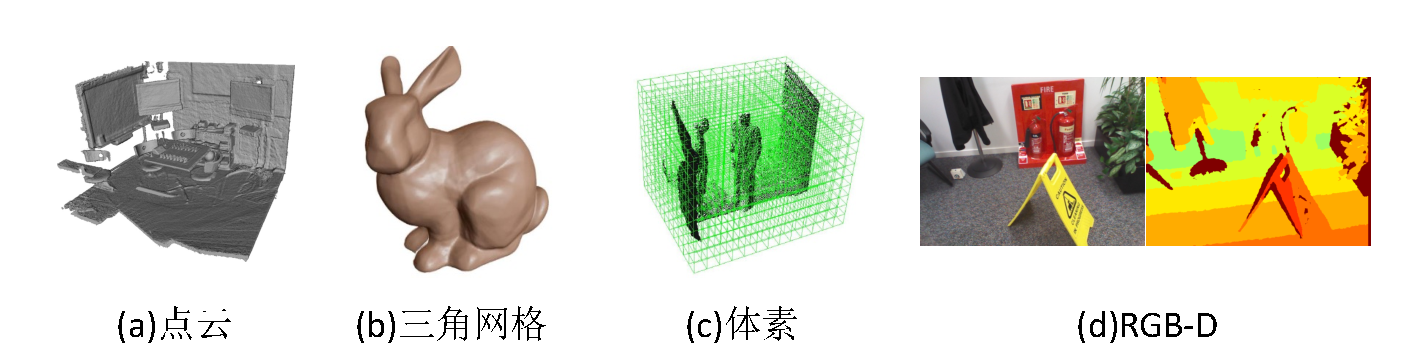
\includegraphics[width=\textwidth]{images/3ddata.pdf}
    \caption{点云、三角网格、体素、深度相机数据可视化示意图}
    \label{fig:3ddata}
    \vspace{-10mm}
\end{figure*}


\subsection{点云数据特点}
点云数据是一种常用的三维数据表征形式,由一系列具有三维坐标(X, Y, Z)的点组成。这些点可以通过激光雷达、结构光传感器、多视角立体视觉等方式采集。点云数据具有以下特点:

1. 无序性:点云数据通常是无序的,即点在数据结构中的顺序并不表示它们在空间中的相对位置。这使得处理点云数据时需要额外关注邻域搜索等问题。

2. 不完整性:由于采集设备的视野限制以及物体遮挡等因素,点云数据往往只能捕捉到物体表面的部分信息,无法完整地描述物体的几何结构。

3. 稀疏性:点云数据在空间中分布可能是不均匀的,有些区域可能点密集,而有些区域可能点稀疏。这会对点云处理算法的性能产生影响。

4. 噪声敏感性:点云数据容易受到测量噪声、环境光照等因素的影响。为了提高数据质量,通常需要对点云进行预处理,如滤波、降采样等。

5. 缺乏拓扑信息:点云数据仅包含物体表面的几何信息,不包含拓扑信息。在需要考虑物体结构的应用场景中,点云数据需要进行进一步处理,如重建三角网格或提取骨架结构等。

6. 可扩展性:点云数据可以方便地扩展以包含其他属性信息,如颜色、法向量、强度等。这有助于提高点云处理算法的性能和鲁棒性。

7. 易于处理和存储:由于点云数据直接表示了物体表面的几何信息,其数据结构简单,便于处理和存储。此外,点云数据可以通过各种数据结构(如KD树、八叉树等)进行高效的组织和检索。

在应用深度学习算法时,由于点云数据的无序性,深度学习算法,比如全连接层、卷积层等无法直接应用于点云数据。因此,需要对点云数据进行预处理,将其转换为有序的数据表征形式,如三角网格\cite{jiang2020local}、体素\cite{guan2020voxel}等。但是这样的方法会造成空间中很多点的浪费,使得输入的数据变得更加稀疏,使得训练数据变少。PointNet\cite{qi2017pointnet}是一种用于处理点云数据的深度学习网络结构,于2017年首次提出。它是一个端到端的神经网络,可以直接从原始点云数据中学习特征表示。PointNet通过使用对称函数(如最大池化)处理输入点云的无序性,同时具有对输入点顺序的不变性。


\subsection{点云特征描述}
三维点云的特征描述,也叫描述子(Descriptor),是一种用于表示点云数据中每个点周围的局部几何特征的向量。描述子捕捉了点云中每个点的几何结构和形状信息,这对于解决诸如点云配准、物体识别、分类和分割等问题至关重要。点云描述子应具有以下特性:鲁棒性、区分性、旋转不变性、尺度不变性和噪声不敏感性。点云描述子对于点云的后处理有着非常巨大的影响,对于不同的任务和数据特征,应该选用合适的描述子来作为网络的预处理。

有许多不同类型的点云描述子,它们根据计算方法和考虑的几何属性而有所不同。以下是一些常见的点云描述子:

1. Spin Images(旋转图像) \cite{johnson1997spin}:通过在点云中每个点周围投影二维图像来表示局部形状信息。

2. Normal Aligned Radial Features(NARF) \cite{steder2010narf}:基于局部表面法线的方向和强度来描述点云中的局部特征。

3. Fast Point Feature Histograms(FPFH) \cite{rusu2009fast}:通过计算每个点周围的点对的几何特征直方图来表示局部特征。

4. Signature of Histograms of Orientations(SHOT) \cite{salti2014shot}:结合局部点的颜色信息和表面法线分布,为每个点计算描述子。

5. Point Pair Features(PPF) \cite{deng2018ppfnet}:描述点云中两个点之间的几何关系,PPF 是一个四元组$(\alpha, d, \theta, \phi)$,其中$\alpha$是两点之间的距离,$d$是两点的法向量之差,$\theta$是两点的法线之间的角度,$\phi$是两点的法线在两点之间连线所确定的平面上的角度。PPF特征在处理点云配准问题时具有很高的鲁棒性,因为它仅依赖于点云的几何信息。

\section{刚体运动参数估计}
刚体运动参数估计是点云配准任务的最后一个阶段的任务。对于位移来说,常用的是位移向量(Transition);旋转的运动参数有不同的表示形式,如欧拉角\cite{pio1966euler}、四元数\cite{shoemake1985animating}、旋转矩阵\cite{horn1954doubly}、轴角\cite{diebel2006representing}等。下面我们对旋转的表示进行简要介绍。

\subsection{旋转矩阵}
旋转矩阵是一种与向量相乘时旋转向量同时保持其长度的矩阵。所有 $3 \times 3$ 旋转矩阵的特殊正交群表示为 $SO(3)$。因此,如果 $\boldsymbol{R} \in SO(3)$,那么
\begin{equation}
\det (\boldsymbol{R}) = \pm1 \quad \text{且} \quad \boldsymbol{R}^{-1} = \boldsymbol{R}^T
\end{equation}

对于满足 $\det (\boldsymbol{R}) = 1$ 的旋转矩阵,称为正规旋转;对于满足 $\det (\boldsymbol{R}) = -1$ 的旋转矩阵,称为非正规旋转。非正规旋转也称为旋转倒数,由旋转后接反演操作组成。我们将分析限制在正规旋转上,因为非正规旋转不是刚体变换。
我们按如下方式引用旋转矩阵的元素:
\begin{align}
    \boldsymbol{R} &=
    \begin{bmatrix}
    r_1 & r_2 & r_3
    \end{bmatrix} \\
    &=
    \begin{bmatrix}
    r_{11} & r_{12} & r_{13} \\
    r_{21} & r_{22} & r_{23} \\
    r_{31} & r_{32} & r_{33}
    \end{bmatrix}
\end{align}

对于正规旋转矩阵,我们可以使用群的定义来进行更精准的定义。
\begin{equation}
    SO(n) = \{\boldsymbol{R} \in \boldsymbol{R}^{n \times n} | \boldsymbol{R}^T\boldsymbol{R} = \boldsymbol{I}, \det (R) = 1\}
\end{equation}
其中,$SO(n)$是特殊正交群 (Special Orthogonal Group),这个集合由$n$维空间的旋转矩阵组成。$SO(n)$是一个群,因为它满足群的四个条件:封闭性、结合律、单位元和逆元。$SO(n)$的单位元是 $\boldsymbol{I}$,逆元是 $\boldsymbol{R}^T$。$SO(n)$的元素称为正规旋转矩阵。通过旋转矩阵可以直接描述相机的旋转。

为了描述两个坐标之间的相对旋转,我们假设某个单位正交基 $\boldsymbol{i}, \boldsymbol{j}, \boldsymbol{k}$,并且我们希望将其旋转到另一个正交基 $\boldsymbol{i}', \boldsymbol{j}', \boldsymbol{k}'$。假设对于同一个向量$\boldsymbol{a} = [a_1, a_2, a_3]^T$,在两个坐标系中的表示分别为 $\boldsymbol{a} = a_1\boldsymbol{i} + a_2\boldsymbol{j} + a_3\boldsymbol{k}$ 和 $\boldsymbol{a}' = a_1'\boldsymbol{i}' + a_2'\boldsymbol{j}' + a_3'\boldsymbol{k}'$,根据坐标的定义,有
\begin{equation}
    [\boldsymbol{i}, \boldsymbol{j}, \boldsymbol{k}] \boldsymbol{a} = [\boldsymbol{i}', \boldsymbol{j}', \boldsymbol{k}'] \boldsymbol{a}'
\end{equation}
我们对上述等式同时左成$[\boldsymbol{i}, \boldsymbol{j}, \boldsymbol{k}]^T$,我们可以通过旋转矩阵 $\boldsymbol{R}$ 来表示两个坐标系之间的旋转关系,即
\begin{equation}
    \boldsymbol{a}' = 
    \begin{bmatrix}
    \boldsymbol{i}^T \boldsymbol{i}' & \boldsymbol{i}^T \boldsymbol{j}' & \boldsymbol{i}^T \boldsymbol{k}' \\
    \boldsymbol{j}^T \boldsymbol{i}' & \boldsymbol{j}^T \boldsymbol{j}' & \boldsymbol{j}^T \boldsymbol{k}' \\
    \boldsymbol{k}^T \boldsymbol{i}' & \boldsymbol{k}^T \boldsymbol{j}' & \boldsymbol{k}^T \boldsymbol{k}'
    \end{bmatrix}
    =
    \boldsymbol{R} \boldsymbol{a}
\end{equation}

因为旋转矩阵是正交矩阵,它的逆就可以用来描述一个相反的旋转,按照上面的推到,则有:
\begin{equation}
    \boldsymbol{a} = \boldsymbol{R}^T \boldsymbol{a}' = \boldsymbol{R}^{-1} \boldsymbol{a}'
\end{equation}

\subsection{欧拉角}
三次坐标旋转依次可以描述任意旋转。我们考虑三次旋转,其中第一次旋转是关于 $\boldsymbol{k}$ 轴的角度 $\psi$,第二次旋转是关于 $\boldsymbol{j}$ 轴的角度 $\theta$,第三次旋转是关于 $\boldsymbol{i}$ 轴的角度 $\phi$,如图 \ref{fig:rotation} (a, b ,c)所示。为了简化符号,我们将这些角度排列成一个三维向量,称为欧拉角向量,定义为 
\begin{equation}
    \boldsymbol{u} := [\phi, \theta, \psi]^T
\end{equation}
将欧拉角向量映射到其对应的旋转矩阵的函数,$\boldsymbol{R}_{ijk} : \boldsymbol{R}^3 \to SO(3)$,定义为
\begin{equation}
    \boldsymbol{R}_{ijk}(\phi, \theta, \psi) := \boldsymbol{R}_i(\phi)\boldsymbol{R}_j(\theta)\boldsymbol{R}_k(\psi)
\end{equation}
与一般情况相同,如果 $\boldsymbol{z} \in R^3$ 是世界坐标系中的一个向量,$\boldsymbol{z}_0 \in R^3$ 是以体固定坐标表示的相同向量,那么以下关系成立:
\begin{equation}
    \boldsymbol{z}_0 = \boldsymbol{R}_{ijk}(\boldsymbol{u}) \boldsymbol{z}
\end{equation}
\begin{equation}
    \boldsymbol{z} = \boldsymbol{R}_{ijk}(\boldsymbol{u})^T \boldsymbol{z}_0
\end{equation}
也就是说,欧拉角并不是定义在三维线性空间的群,欧拉角的相互转换需要借助旋转矩阵来进行表达。

\begin{figure}
    \centering
    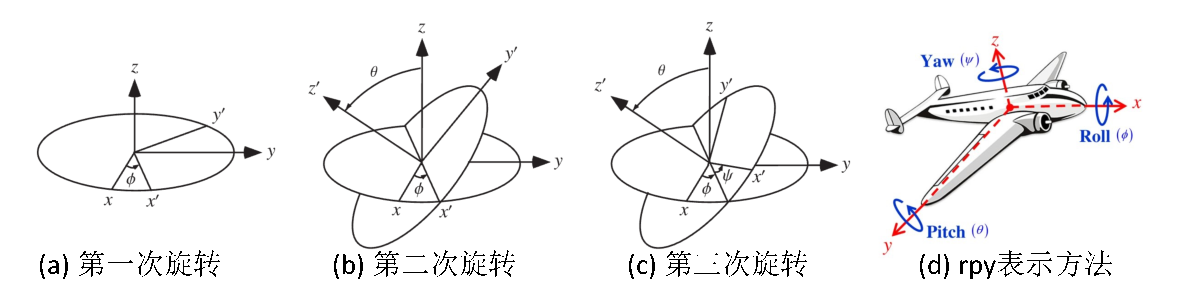
\includegraphics[width=0.8\textwidth]{images/rotation.pdf}
    \caption{欧拉角旋转表示}
    \label{fig:rotation}
\end{figure}

在自动化或者航空航天领域比较常用的欧拉角的分解方式是 $Z-Y-X$,也就是说,先绕 $z$ 轴旋转 $\psi$ 角,然后绕 $y$ 轴旋转 $\theta$ 角,最后绕 $x$ 轴旋转 $\phi$ 角。这种分解方式也被称为航空分解(Aerospace decomposition),通常这种方式中的$Z-Y-X$会被称为“偏航 - 俯仰 - 旋转 (yaw - pitch - roll)”。在这种分解方式中,欧拉角向量的顺序是 $\boldsymbol{u} = [\psi, \theta, \phi]^T$,如图 \ref{fig:rotation} (d)所示。

欧拉角的一个缺点是会碰到著名的万象锁问题\cite{vsenk2006rotation},也就是说,当 $\theta = \pm \frac{\pi}{2}$ 时,旋转矩阵 $\boldsymbol{R}_{ijk}(\boldsymbol{u})$ 的值会变成奇异的。理论上可以证明,只要想要用3个数来表达三位旋转时,基本都会碰到奇异性问题\cite{stuelpnagel1964parametrization}。由于这种原理,欧拉角不适用于迭代和插值,在传统的SLAM中和深度学习中几乎都不会是用这种方式来进行迭代,但是欧拉角对于人机交互是友好的。

\subsection{四元数}
旋转矩阵使用了9个未知数来描述3自由度的旋转,这在数学表达上具有冗余性了;欧拉角使用了3个未知数来描述3自由度的旋转,在数学表达上是紧凑的,但是具有奇异性。因为我们找不到不带奇异性,且使用3个未知数的方法来描述3维旋转的描述方式\cite{stuelpnagel1964parametrization}。这个性质,可以类比于用两个坐标描述地球表面(二维流形)上的点,我们可以使用经纬度来描述地球表面上的点,但是在极点处,经纬度的表达就会出现奇异性,即纬度为$\pm 90^{\circ}$时,经度无意义。

三位旋转是一个三维流形,因此,为了最优平衡无奇异性和数学表达的紧凑性,我们需要引入一个新的数学工具来描述3自由度的旋转,这个数学工具就是四元数。四元数是Hamilton找到的一种超复数,它在数学形式上既是紧凑的,又是非奇异的。四元数的定义如下:
\begin{equation}
    \boldsymbol{q} = q_0 + q_1 i + q_2 j + q_3 k
\end{equation}
其中,$q_0, q_1, q_2, q_3 \in R$,$i, j, k$ 是四元数的三个虚数单位,满足如下关系:
\begin{equation}
    \left\{
    \begin{aligned}
        &i^2 = j^2 = k^2 = ijk = -1, \\
        &ij = k, jk = i, ki = j, \\
        &ji = -k, kj = -i, ik = -j
    \end{aligned}
    \right.
\end{equation}
假设某个旋转是绕着单位向量 $\boldsymbol{u} = [u_x, u_y, u_z]^T$ 旋转 $\theta$ 角,那么这个旋转可以用四元数来表示为:
\begin{equation}
    \boldsymbol{q} = \cos \frac{\theta}{2} + \sin \frac{\theta}{2} (u_x i + u_y j + u_z k)
\end{equation}
同时,我们也可以从单位四元数种计算出对应的旋转轴和旋转角:
\begin{equation}
    \left\{
    \begin{aligned}
        &\theta = 2 \arccos q_0, \\
        &u_x = \frac{q_1}{\sin \frac{\theta}{2}}, u_y = \frac{q_2}{\sin \frac{\theta}{2}}, u_z = \frac{q_3}{\sin \frac{\theta}{2}}
    \end{aligned}
    \right.
\end{equation}

因为四元数是定义在复向量空间中而非旋转流形中,并且四元数没有死锁的特性,所以在深度学习的梯度下降算法中,常常用四元数作为回归的目标。并且,因为三维流形的性质,我们在四元数中同乘一个常数,可以得到相同的旋转,即$[q_0, q_1, q_2, q_3] \iff k[q_0, q_1, q_2, q_3]$。由于这个性质,在回归任务中,我们通常回归单位四元数,即$\sum_0^3 q_i^2 = 1$。

{\bf 用四元数表示旋转。} 用四元数同样也可以表达对一个点的旋转,假设一个空间中的三维坐标点为$\boldsymbol{a} = [x, y, z] \in \mathbb{R}^3$。以及一个旋转轴$\boldsymbol{n}$和旋转角$\theta$,这个点绕着旋转轴旋转$\theta$角后的坐标为$\boldsymbol{a}'$,则:
\begin{equation}
    \boldsymbol{p}' = \boldsymbol{Rp} = \boldsymbol{qpq}^{-1}
\end{equation}
其中,$\boldsymbol{q} = [\cos \frac{\theta}{2}, \boldsymbol{n} \sin \frac{\theta}{2}]$。

\subsection{基于奇异值分解的线性代数求解}
奇异值分解\cite{levinson2020analysis} (Singular Value Decomposition, SVD) 是线性代数中一种重要的矩阵分解,在信号处理、计算机视觉、运动估计中有着非常广泛的运用。下面,我们对奇异值分解的线性代数部分进行简要介绍。

奇异值分解对一个矩形数据矩阵(定义为$\boldsymbol{A}$,其中$\boldsymbol{A}$是一个$n \times p$矩阵)进行处理,其中n行代表观察值,p列代表变量。SVD定理如下:

\begin{equation}
\boldsymbol{A}_{n \times p} = \boldsymbol{U}_{n \times n} \boldsymbol{S}_{n \times p} \boldsymbol{V}^T_{p \times p}
\end{equation}
其中

\begin{equation}
\boldsymbol{U}^T \boldsymbol{U} = \boldsymbol{I}_{n \times n}
\end{equation}

\begin{equation}
\boldsymbol{V}^T \boldsymbol{V} = \boldsymbol{I}_{p \times p}
\end{equation}

即$\boldsymbol{U}$和$\boldsymbol{V}$是正交的。$\boldsymbol{U}$的列是左奇异向量(观察值系数向量);$\boldsymbol{S}$(与$\boldsymbol{A}$的维度相同)具有奇异值,并且是对角的(模振幅);$\boldsymbol{V}^T$的行是右奇异向量(变量水平向量)。SVD表示了原始数据在协方差矩阵为对角线的坐标系中的扩展。

计算SVD包括寻找$\boldsymbol{A} \boldsymbol{A}^T$和$\boldsymbol{A}^T \boldsymbol{A}$的特征值和特征向量。$\boldsymbol{A}^T \boldsymbol{A}$的特征向量构成$\boldsymbol{V}$的列,$\boldsymbol{A} \boldsymbol{A}^T$的特征向量构成$\boldsymbol{U}$的列。此外,$\boldsymbol{S}$中的奇异值是来自$\boldsymbol{A} \boldsymbol{A}^T$或$\boldsymbol{A}^T \boldsymbol{A}$的特征值的平方根。奇异值是$\boldsymbol{S}$矩阵的对角线条目,并按降序排列。奇异值总是实数。如果矩阵$\boldsymbol{A}$是实数矩阵,那么$\boldsymbol{U}$和$\boldsymbol{V}$也是实数。

奇异值分解(SVD)在点云配准问题中也具有重要应用。点云配准是将两个或多个点云数据集合并为一个统一坐标系的过程。在这种情况下,我们的目标是找到一个最优的刚体变换,包括旋转和平移,使得两个点云之间的距离最小化。

假设我们有两个点云数据集$\boldsymbol{P}$和$\boldsymbol{Q}$,每个点云包含$n$个点。我们首先计算两个点云的质心$\boldsymbol{p}_c$和$\boldsymbol{q}_c$,然后将点云平移到原点。接下来,我们计算点云$\boldsymbol{P}$和$\boldsymbol{Q}$之间的距离矩阵$\boldsymbol{H}$,其中$\boldsymbol{H}=\boldsymbol{P}^T\boldsymbol{Q}$。

在这种情况下,我们可以使用SVD来求解最优的旋转矩阵$\boldsymbol{R}$,使得两个点云之间的距离最小化。具体来说,我们对距离矩阵$\boldsymbol{H}$进行奇异值分解:

\begin{equation}
\boldsymbol{H} = \boldsymbol{U} \boldsymbol{S} \boldsymbol{V}^T
\end{equation}

然后,我们计算旋转矩阵$\boldsymbol{R}$:

\begin{equation}
\boldsymbol{R} = \boldsymbol{U} \boldsymbol{V}^T
\end{equation}

如果$\boldsymbol{R}$是一个不合适的旋转矩阵(即$\det(\boldsymbol{R})\neq 1$),我们可以通过修改$\boldsymbol{S}$矩阵来修复它。具体而言,我们将$\boldsymbol{S}$的最小奇异值设为$-1$,然后重新计算旋转矩阵$\boldsymbol{R}$。

最后,我们可以计算最优的平移向量$\boldsymbol{t}$:

\begin{equation}
\boldsymbol{t} = \boldsymbol{q}_c - \boldsymbol{R} \boldsymbol{p}_c
\end{equation}

通过应用旋转矩阵$\boldsymbol{R}$和平移向量$\boldsymbol{t}$,我们可以将点云$\boldsymbol{P}$对齐到点云$\boldsymbol{Q}$,从而实现点云配准。

\subsection{基于Levenberg-Marquardt算法的非线性优化求解}
在数学和计算领域,Levenberg-Marquardt算法(LMA或简称LM)\cite{levenberg1944method},也称为阻尼最小二乘法(DLS),用于求解非线性最小二乘问题。这些最小化问题尤其出现在最小二乘曲线拟合中。LMA在高斯-牛顿算法(GNA)\cite{}和梯度下降法之间进行插值。LMA比GNA更稳健,这意味着在许多情况下,即使它从距离最终最小值非常远的地方开始,也能找到解决方案。对于行为良好的函数和合理的初始参数,LMA往往比GNA慢。LMA也可以被视为使用信任区域方法的高斯-牛顿算法。

需要LM算法求解的问题被称为非线性最小二乘最小化问题。这意味着要最小化的函数具有以下特殊形式:

\begin{equation}
f(x) = \frac{1}{2} \sum_{j=1}^{m} r_j^2(x)
\end{equation}

其中 $x = (x_1, x_2, \dots, x_n)^T$ 是一个向量,每个 $r_j$ 是一个从 $\mathbb{R}^n$ 到 $\mathbb{R}$ 的函数。$r_j$ 被称为残差,并且假定 $m \geq n$。

为了简化问题,我们用残差向量 $r : \mathbb{R}^n \rightarrow \mathbb{R}^m$ 来表示 $f$,定义为:

\begin{equation}
r(x) =
\begin{bmatrix}
r_1(x) \
r_2(x) \
\cdots \
r_m(x)
\end{bmatrix}
\end{equation}

现在,$f$ 可以重写为 $f(x) = \frac{1}{2} ||r(x)||^2$。$f$ 的导数可以用相对于 $x$ 的 $r$ 的雅可比矩阵 $J(x)$ 来表示,定义为 $J(x) = \frac{\partial r_j}{\partial x_i}$,其中 $1 \leq j \leq m$,$1 \leq i \leq n$。

首先考虑线性情况,其中每个 $r_i$ 函数都是线性的。在这里,雅可比矩阵是常数,我们可以将 $r$ 表示为空间中的超平面,这样 $f$ 给出二次型:

\begin{equation}
f(x) = \frac{1}{2} ||Jx - r_0||^2
\end{equation}

我们还得到 $\nabla f(x) = J^T(Jx - r_0)$ 和 $\nabla^2 f(x) = J^TJ$。通过将 $\nabla f(x) = 0$ 求解最小值,我们得到 $x_\text{min} = (J^TJ)^{-1}J^Tr$,这是一组无约束优化问题的解。

回到一般的非线性情况,我们有:

\begin{equation}
\nabla f(x) = J(x)^T r(x)
\label{eq:grad}
\end{equation}

\begin{equation}
\nabla^2 f(x) = J(x)^TJ(x) + \sum_{j=1}^{m} r_j(x) \nabla^2 r_j(x)
\label{eq:hessian}
\end{equation}

最小二乘问题的独特属性是,给定雅可比矩阵 $J$,如果可以将 $r_j$ 用线性函数近似($\nabla^2 r_j(x)$ 较小)或残差 $r_j(x)$ 本身较小,我们可以实质上免费获得海森矩阵($\nabla^2 f(x)$)。在这种情况下,海森矩阵简化为:

\begin{equation}
\nabla^2 f(x) = J(x)^T J(x)
\label{eq:hessian_approx}
\end{equation}

这与线性情况相同。这里通常使用的近似是在解附近的 $r_i$ 近似线性,这样 $\nabla^2 r_j(x)$ 较小。还要注意,只有在残差较小时,式 \ref{eq:hessian_approx} 才有效。对于大残差问题,不能使用二次近似求解\cite{李娇娇2022基于深度学习的}。

考虑到点云配准问题,我们可以将 Levenberg-Marquardt 算法应用于点云之间的非线性最小二乘优化问题。在这种情况下,我们寻求最小化点云之间的距离,同时考虑旋转和平移变换。通过迭代地优化变换参数,Levenberg-Marquardt 算法可以在点云配准问题中找到一个稳定的解决方案。


\section{标准数据集}
\subsection{ModelNet40}
\subsection{ShapeNet}
\subsection{Scan2CAD}

\section{点云配准评价指标}
\subsection{基于特征提取与匹配的评价指标}
\subsection{基于刚体运动的评价指标}
\subsection{多实例点云配准评价指标}

\section{点云处理与配准相关深度学习技术}
\subsection{深度学习概述}
\subsection{多层感知机}
\subsection{卷积神经网络}
\subsubsection{三维卷积神经网络}
\subsubsection{点云卷积神经网络}
\subsection{注意力机制}
\subsection{谱聚类算法}

\section{小结}

\begin{lstlisting}[language=Python, caption={Python Code}, label={lst:pythonfile}]
import numpy as np

def incmatrix(genl1,genl2):
    m = len(genl1)
    n = len(genl2)
    M = None #to become the incidence matrix
    VT = np.zeros((n*m,1), int)  #dummy variable

    #compute the bitwise xor matrix
    M1 = bitxormatrix(genl1)
    M2 = np.triu(bitxormatrix(genl2),1)

    for i in range(m-1):
        for j in range(i+1, m):
            [r,c] = np.where(M2 == M1[i,j])
            for k in range(len(r)):
                VT[(i)*n + r[k]] = 1;
                VT[(i)*n + c[k]] = 1;
                VT[(j)*n + r[k]] = 1;
                VT[(j)*n + c[k]] = 1;

                if M is None:
                    M = np.copy(VT)
                else:
                    M = np.concatenate((M, VT), 1)

                VT = np.zeros((n*m,1), int)

    return M
\end{lstlisting}

% %%
% The BIThesis Template for Bachelor Paper Translation
%
% 北京理工大学毕业设计(论文) —— 使用 XeLaTeX 编译
%
% Copyright 2020-2023 BITNP
%
% This work may be distributed and/or modified under the
% conditions of the LaTeX Project Public License, either version 1.3
% of this license or (at your option) any later version.
% The latest version of this license is in
%   http://www.latex-project.org/lppl.txt
% and version 1.3 or later is part of all distributions of LaTeX
% version 2005/12/01 or later.
%
% This work has the LPPL maintenance status `maintained'.
%
% The Current Maintainer of this work is Feng Kaiyu.
%
% Compile with: xelatex -> biber -> xelatex -> xelatex
%%

% 第一章节

\chapter{问题陈述}


在多实例点云配准问题中,源点云$\mathbf{X}$提供了一个3D模型的实例,目标点云$\mathbf{Y}$包含了这个模型的$K$个实例,其中这些实例是一组点的集合,这些点可能只采样了3D模型的一部分。如果我们将第$k^{th}$个实例写为$\mathbf{Y}_k$,那么目标点云$\mathbf{Y}$可以分解为$
%\begin{equation}
\mathbf{Y} = \mathbf{Y}_0 \cup \mathbf{Y}_1 \cup \ldots \mathbf{Y}_k \ldots \cup \mathbf{Y}_K$。
%\end{equation}
这里我们使用$\mathbf{Y}_0$表示点云中不属于任何实例的部分。
多实例3D配准的目标是找到刚性变换$(\mathbf{R}_k, \mathbf{t}_k)$,将源实例$\mathbf{X}$对准到每个目标实例$\mathbf{Y}_k$。
如果我们设法获得源实例与每个目标实例$\mathbf{X} \leftrightarrow \mathbf{Y}_k$之间的对应关系,那么通过最小化对齐误差之和(\ref{eq:solve_rigid_transform}) \cite{SVD},可以从对应关系集合$\mathbf{X}\leftrightarrow \mathbf{Y}_k$中求解目标点云中第$k^{th}$个实例的位姿$(\mathbf{R}_k, \mathbf{t}_k)$:
\begin{equation}
\underset{\mathbf{R}_k,\mathbf{t}k}{\min}\sum_i{\parallel}\mathbf{y}{ki}-(\mathbf{R}_k\mathbf{x}_i+\mathbf{t}_k)\parallel ^2.
\label{eq:solve_rigid_transform}
\end{equation}
考虑到我们已经获得了源点云和目标点云之间的一组对应关系$\mathcal{C}$。多实例配准任务的关键是将这些对应关系分类为与不同实例相关的独立集合,即:
\begin{equation}
\mathcal{C} = \mathcal{C}_0 \cup \mathcal{C}_1\cdots \cup \mathcal{C}_K.
\end{equation}
这里,$\mathcal{C}_0$用来表示异常值集合。如我们所见,多实例配准不仅需要剔除异常值对应关系,还需要解决来自不同实例的对应关系的歧义。这个任务并不容易,因为所有实例看起来都一样,而且通常存在大量的异常值对应关系。












% 后置部分
\backmatter

% 结论:在结论相应的 TeX 文件处进行结论部分的撰写
%%
% The BIThesis Template for Bachelor Graduation Thesis
%
% 北京理工大学毕业设计(论文)结论 —— 使用 XeLaTeX 编译
%
% Copyright 2020-2023 BITNP
%
% This work may be distributed and/or modified under the
% conditions of the LaTeX Project Public License, either version 1.3
% of this license or (at your option) any later version.
% The latest version of this license is in
%   http://www.latex-project.org/lppl.txt
% and version 1.3 or later is part of all distributions of LaTeX
% version 2005/12/01 or later.
%
% This work has the LPPL maintenance status `maintained'.
%
% The Current Maintainer of this work is Feng Kaiyu.
%
% Compile with: xelatex -> biber -> xelatex -> xelatex

\begin{conclusion}
  % 结论部分尽量不使用 \subsection 二级标题,只使用 \section 一级标题

  % 这里插入一个参考文献,仅作参考
\end{conclusion}


% 参考文献:如无特殊需要,参考文献相应的 TeX 文件无需改动,添加参考文献请使用 BibTeX 的格式
%   添加至 misc/ref.bib 中,并在正文的相应位置使用 \cite{xxx} 的格式引用参考文献
%%
% The BIThesis Template for Bachelor Graduation Thesis
%
% 北京理工大学毕业设计(论文)参考文献 —— 使用 XeLaTeX 编译
%
% Copyright 2020-2023 BITNP
%
% This work may be distributed and/or modified under the
% conditions of the LaTeX Project Public License, either version 1.3
% of this license or (at your option) any later version.
% The latest version of this license is in
%   http://www.latex-project.org/lppl.txt
% and version 1.3 or later is part of all distributions of LaTeX
% version 2005/12/01 or later.
%
% This work has the LPPL maintenance status `maintained'.
%
% The Current Maintainer of this work is Feng Kaiyu.
%
% Compile with: xelatex -> biber -> xelatex -> xelatex
%
% 如无特殊需要,本页面无需更改

\begin{bibprint}

% -------------------------------- 示例内容(正式使用时请删除) ------------------------------------- %

% 抑制多次调用 \printbibliography 的 warning,只有示例代码会需要此语句。
\BiblatexSplitbibDefernumbersWarningOff

% \textcolor{blue}{参考文献书写规范}

% \textcolor{blue}{参考国家标准《信息与文献参考文献著录规则》【GB/T 7714—2015】,参考文献书写规范如下:}

% \textcolor{blue}{\textbf{1. 文献类型和标识代码}}

% \textcolor{blue}{普通图书:M}\qquad\textcolor{blue}{会议录:C}\qquad\textcolor{blue}{汇编:G}\qquad\textcolor{blue}{报纸:N}

% \textcolor{blue}{期刊:J}\qquad\textcolor{blue}{学位论文:D}\qquad\textcolor{blue}{报告:R}\qquad\textcolor{blue}{标准:S}

% \textcolor{blue}{专利:P}\qquad\textcolor{blue}{数据库:DB}\qquad\textcolor{blue}{计算机程序:CP}\qquad\textcolor{blue}{电子公告:EB}

% \textcolor{blue}{档案:A}\qquad\textcolor{blue}{舆图:CM}\qquad\textcolor{blue}{数据集:DS}\qquad\textcolor{blue}{其他:Z}

% \textcolor{blue}{\textbf{2. 不同类别文献书写规范要求}}

% \textcolor{blue}{\textbf{期刊}}

% \noindent\textcolor{blue}{[序号]主要责任者. 文献题名[J]. 刊名, 出版年份, 卷号(期号): 起止页码. }

% \printbibliography [type=article,heading=none] 

% \textcolor{blue}{\textbf{普通图书}}

% \noindent\textcolor{blue}{[序号]主要责任者. 文献题名[M]. 出版地: 出版者, 出版年. 起止页码. }
% \cite{Raymer1992Aircraft}

% \printbibliography [keyword={book},heading=none] 

% \textcolor{blue}{\textbf{会议论文集}}

% \noindent\textcolor{blue}{[序号]析出责任者. 析出题名[A]. 见(英文用In): 主编. 论文集名[C]. (供选择项: 会议名, 会址, 开会年)出版地: 出版者, 出版年. 起止页码. }
% \cite{sunpinyi}

% \printbibliography [type=inproceedings,heading=none] 

% \textcolor{blue}{\textbf{专著中析出的文献}}

% \noindent\textcolor{blue}{[序号]析出责任者. 析出题名[A]. 见(英文用In): 专著责任者. 书名[M]. 出版地: 出版者, 出版年.起止页码. }
% \cite{luoyun}

% \printbibliography [type=inbook,heading=none] 

% \textcolor{blue}{\textbf{学位论文}}

% \noindent\textcolor{blue}{[序号]主要责任者. 文献题名[D]. 保存地: 保存单位, 年份. }
% \cite{zhanghesheng}
% \cite{Sobieski}

% \printbibliography [keyword={thesis},heading=none] 

% \textcolor{blue}{\textbf{报告}}

% \noindent\textcolor{blue}{[序号]主要责任者. 文献题名[R]. 报告地: 报告会主办单位, 年份. }
% \cite{fengxiqiao}
% \cite{Sobieszczanski}

% \printbibliography [keyword={techreport},heading=none] 

% \textcolor{blue}{\textbf{专利文献}}

% \noindent\textcolor{blue}{[序号]专利所有者. 专利题名[P]. 专利国别: 专利号, 发布日期. }
% \cite{jiangxizhou}

% \printbibliography [type=patent,heading=none] 

% \textcolor{blue}{\textbf{国际、国家标准}}

% \noindent\textcolor{blue}{[序号]标准代号. 标准名称[S]. 出版地: 出版者, 出版年. }
% \cite{GB/T16159—1996}

% \printbibliography [keyword={standard},heading=none] 

% \textcolor{blue}{\textbf{报纸文章}}

% \noindent\textcolor{blue}{[序号]主要责任者. 文献题名[N]. 报纸名, 出版年, 月(日): 版次. }
% \cite{xiexide}

% \printbibliography [keyword={newspaper},heading=none] 

% \textcolor{blue}{\textbf{电子文献}}

% \noindent\textcolor{blue}{[序号]主要责任者. 电子文献题名[文献类型/载体类型]. 电子文献的出版或可获得地址(电子文献地址用文字表述), 发表或更新日期/引用日期(任选). }
% \cite{yaoboyuan}

% \printbibliography [keyword={online},heading=none] 

% \textcolor{blue}{关于参考文献的未尽事项可参考国家标准《信息与文献参考文献著录规则》(GB/T 7714—2015)}

% 在使用时,请删除/注释上方示例内容,并启用下方语句以输出所有的参考文献
\printbibliography[heading=none]
\end{bibprint}

% 附录:在附录相应的 TeX 文件处进行附录部分的撰写
%%
% The BIThesis Template for Bachelor Graduation Thesis
%
% 北京理工大学毕业设计(论文)附录 —— 使用 XeLaTeX 编译
%
% Copyright 2020-2023 BITNP
%
% This work may be distributed and/or modified under the
% conditions of the LaTeX Project Public License, either version 1.3
% of this license or (at your option) any later version.
% The latest version of this license is in
%   http://www.latex-project.org/lppl.txt
% and version 1.3 or later is part of all distributions of LaTeX
% version 2005/12/01 or later.
%
% This work has the LPPL maintenance status `maintained'.
%
% The Current Maintainer of this work is Feng Kaiyu.
%
% Compile with: xelatex -> biber -> xelatex -> xelatex

\begin{appendices}
  附录相关内容…

  % 这里示范一下添加多个附录的方法:
  % 使用 \section 来添加一个附录

  \section{\LaTeX 环境的安装}
  \LaTeX 环境的安装。

  \section{BIThesis 使用说明}
  BIThesis 使用说明。

  \textcolor{blue}{附录是毕业设计(论文)主体的补充项目,为了体现整篇文章的完整性,写入正文又可能有损于论文的条理性、逻辑性和精炼性,这些材料可以写入附录段,但对于每一篇文章并不是必须的。附录依次用大写正体英文字母 A、B、C……编序号,如附录 A、附录 B。阅后删除此段。}

  \textcolor{blue}{附录正文样式与文章正文相同:宋体、小四;行距:22 磅;间距段前段后均为 0 行。阅后删除此段。}

\end{appendices}


% 致谢:在致谢相应的 TeX 文件处进行致谢部分的撰写
%%
% The BIThesis Template for Bachelor Graduation Thesis
%
% 北京理工大学毕业设计(论文)致谢 —— 使用 XeLaTeX 编译
%
% Copyright 2020-2023 BITNP
%
% This work may be distributed and/or modified under the
% conditions of the LaTeX Project Public License, either version 1.3
% of this license or (at your option) any later version.
% The latest version of this license is in
%   http://www.latex-project.org/lppl.txt
% and version 1.3 or later is part of all distributions of LaTeX
% version 2005/12/01 or later.
%
% This work has the LPPL maintenance status `maintained'.
%
% The Current Maintainer of this work is Feng Kaiyu.
%
% Compile with: xelatex -> biber -> xelatex -> xelatex

% 致谢部分尽量不使用 \subsection 二级标题,只使用 \section 一级标题
\begin{acknowledgements}
% 首先,我要对我科研旅程的引路人,曾祥远教授和由育阳教授表示深深的感谢。他们的悉心指导和无私帮助让我能在学习和科研上都取得了长足的进步。

% 我还要对带领我进入计算机视觉领域的赵昊教授和石永亮博士表示衷心的感谢。在与他们一年的合作过程中,我的科研能力有了突飞猛进的提升,这是我无法忘记的宝贵经历。在清华大学智能产业研究院实习的一年,是我学习到最多东西的一年,也结识了很多优秀的朋友,感谢学术路上有你们一同前行。

% 对于在我毕业设计过程中给予我无私帮助和宝贵建议的由育阳教授和钟程亮博士,我表示深深的感激。他们的专业精神和严谨态度让我深受启发。

% 此外,我还要对陪我走过高中以来的两位挚友孟繁禹和谢扬表示诚挚的感谢。他们在我求学之路上给予了我巨大的支持和帮助,我也要感谢所有曾经帮助过我的朋友们,没有你们的帮助我无法达到今天的成就。

% 最后,我要对我的女朋友许舒蕾表示深深的感激。她在我求学过程中对我无比的支持和理解,对我在申请过程中的帮助让我感到无比温暖。我为有她为伴而感到无比的幸福。
\end{acknowledgements}


\end{document}
